
\begin{frame}
 \frametitle{Demo 7-1 $\vert$ \bfseries Thermo-elasticity}
 \framesubtitle{\bfseries bimetallic thermometer}
 \begin{overlayarea}{0.9\textwidth}{0.9\textheight}
%  \vspace*{1ex}
 \begin{center}
 \begin{tikzpicture}[scale=2]
  \onslide<1>{
    \fill[gray!50] (0.0, 0.0) rectangle +(-0.05, 0.4);
  \fill[gray!50] (4.0, 0.0) rectangle +(0.05, 0.4);
  \fill[gray!50] (-0.05, 0.0) rectangle +(4.1, -0.05);
  \fill[gray!50] (-0.05, 0.4) rectangle +(4.1, 0.05);
  
  \fill[gray!10, draw=black] (0, 0.4) rectangle (4, 0) node[above left, yshift=-2pt, black]{$\mathcal{B}$};
  }

  \onslide<1>{
  \draw[thin,gray] (0, 0) -- +(0, -0.5);
  \draw[thin,gray] (4, 0) -- +(0, -0.5);
  \draw[<->,thin,gray] (0, -0.4) -- node[fill=white]{$3 \, \mathrm{cm}$} +(4, 0);
  \draw[thin,gray] (4, 0) -- +(0.5, 0);
  \draw[thin,gray] (4, 0.4) -- +(0.5, -0);
  \draw[<->,gray] (4.4, 0) -- node[fill=white]{$2 \, \mathrm{mm}$} +(0, 0.4);

   \draw[thick,-latex] (0,0) -- +(0.5, 0) node[below]{$\v e_1$};
   \draw[thick,-latex] (0,0) -- +(0, 0.5) node[right]{$\v e_2$};
  }
  
%   \onslide<1>{
%   \foreach \x in {0.0, 0.25,0.5,...,2.75, 3.0}{
%    \draw[decorate,decoration={snake, amplitude=1pt, segment length=5pt, post length=3pt},-latex] (0.05+2.9/3.0*\x, 1.5) -- +(0, -0.5);
%    \draw[decorate,decoration={snake, amplitude=1pt, segment length=5pt, post length=3pt},-latex] (0.05+2.9/3.0*\x, 0.0) -- +(0, -0.5);  
%   }
% %   \draw (0.05, 1.5) -- node[above]{$10 \,\mathrm{MPa}$} +(2.9, 0);
%   \node at (2.9, 1.5) [right,xshift=0.1cm]{$q^p_\text{top}$};
%   \node at (2.9, -0.5) [right,xshift=0.1cm]{$q^p_\text{bottom}$};
%   }

%   \onslide<2>{
%   \node at(2,-0.15) {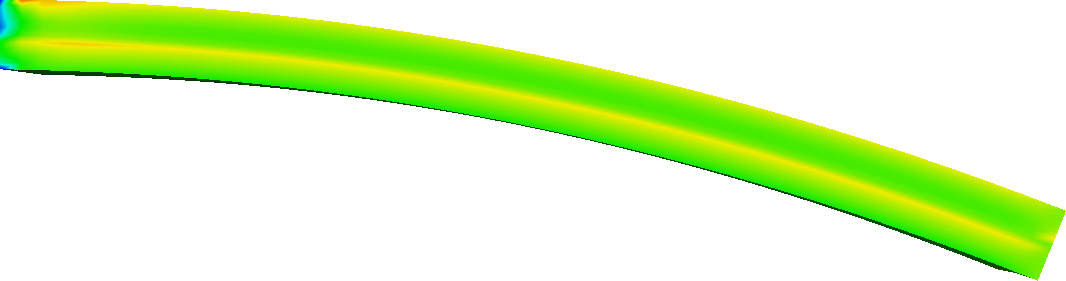
\includegraphics[width=8cm]{../03-thermo-elasto-static/02-bimetal/stress.png}};
%   \begin{scope}[xshift=4cm,yshift=0.8cm,scale=0.5]
%    \begin{axis}[stressbar,point meta min=-110,point meta max=67,title={$\sigma_{11}$ in $\mathrm{MPa}$}] 
%     \addplot [draw=none] coordinates {(0,0)}; \end{axis}
%   \end{scope}   
%   }

  \onslide<1>{
  \fill[pattern=north west lines, pattern color=black] (0, -0.25) rectangle +(-0.25, 0.9);
  \draw[thick] (0, -0.25) -- +(0, 0.9);
%   \fill[pattern=north west lines, pattern color=black] (3, -0.25) rectangle +(0.25, 1.5);
%   \draw[thick] (3, -0.25) -- +(0, 1.5);
  }
  \onslide<1>{
   \draw[dashed] (0, 0.2) -- +(4, 0);
   \node at (2, 0.3) {$\alpha_1$};
   \node at (2, 0.1) {$\alpha_2$};
   
   \node at (1.2, 0.4) [above]{$\theta^p = \theta_0 + \frac{t}{T} \cdot 25 \, \mathrm{K}$};
   \node at (2.8, 0.0) [below]{$\theta^p = \theta_0 + \frac{t}{T} \cdot 25 \, \mathrm{K}$};

 }

  
  \begin{scope}
   \onslide<1>{\node at (0, -1.5) [right]{\parbox{3cm}{
  	    $E = 200 \, \mathrm{GPa}$ \\ $\nu = 0.3$ \\ $\rho = 8000 \, \frac{\mathrm{kg}}{\mathrm{m}^3}$ \\
	    $\kappa = 80 \, \frac{\mathrm{W}}{\mathrm{m}\cdot\mathrm{K}}$ \\[0.5ex] \hspace*{-0.7em} $c_v = 3.2 \, \tfrac{\mathrm{MW}}{\mathrm{m}^3 \cdot \mathrm{K}}$
	    }};}
   \onslide<1>{\node at (1.5, -1.45) [right]{\parbox{3cm}{$\alpha_1 = 15\cdot 10^{-6} \, \frac{1}{\mathrm{K}}$\\
							 $\alpha_2 = 1\cdot 10^{-6} \, \frac{1}{\mathrm{K}}$ \\[4ex]
							 $\theta^p = \theta_0 + \frac{t}{T} \cdot 25 \, \mathrm{K}$ \\
							 $T = 10 \, \mathrm{s}$
							 }};}
%    \onslide<1>{\node at (3.2, -1.5) [right]{\parbox{4cm}{$q^p_\text{top} = 10 \, \frac{\mathrm{kW}}{\mathrm{m}^2}$ \\ 
% 							 $q^p_\text{bottom} = -10 \, \frac{\mathrm{kW}}{\mathrm{m}^2}$}};}
%    \onslide<2>{\node at (0, -0.5) [right,font=\footnotesize]{$\v u$ scaled with a factor of $50$};}
  \end{scope}
  
  \onslide<1>{
   \node at(4.5,-1.3) {
\includegraphics[width=3cm]{thermometer.jpg}};
   \node at(4.5,-2.1) {\parbox{3cm}{\tiny https://commons.wikimedia.org \\/w/index.php?curid=235662\\ CC BY-SA 3.0}};
  }
  
  \end{tikzpicture}
  \end{center}

 \end{overlayarea}
\end{frame}


\begin{frame}
 \frametitle{Demo 7-2 $\vert$ \bfseries Thermo-elasticity}
 \framesubtitle{\bfseries Gough-Joule effect}
 \begin{overlayarea}{0.9\textwidth}{0.9\textheight}
%   \vspace*{3ex}
 \begin{center}
 \begin{tikzpicture}
  \begin{scope}[scale=1.8]
  \onslide<1>{
  \fill[gray!10, draw=black] (0, 1) rectangle (4, 0) node[above left, black]{$\mathcal{B}$};
  }

  \onslide<1>{
  \draw[thin,gray] (0, 0) -- +(0, -0.5);
  \draw[thin,gray] (4, 0) -- +(0, -0.5);
  \draw[<->,thin,gray] (0, -0.4) -- node[fill=white]{$4 \ell$} +(4, 0);
  \draw[thin,gray] (0, 0) -- +(-0.75, 0);
  \draw[thin,gray] (0, 1) -- +(-0.75, -0);
  \draw[<->,gray] (-0.65, 0) -- node[fill=white,sloped]{$\ell$} +(0, 1);

   \draw[thick,-latex] (0,0) -- +(0.5, 0) node[below]{$\v e_1$};
   \draw[thick,-latex] (0,0) -- +(0, 0.5) node[right]{$\v e_2$};
  }
  
  \onslide<1>{
  \foreach \y in {0.0, 0.25, 0.5,..., 1.0}
   \draw[-latex] (4.0, \y) -- +(0.5, 0.0);  
   \node at (4.5, 1.0) [right,xshift=0.1cm]{$\v t^p$};
  }

 \onslide<1>{
  \fill[pattern=north west lines, pattern color=black] (0, -0.25) rectangle +(-0.25, 1.5);
  \draw[thick] (0, -0.25) -- +(0, 1.5);
  }
  \end{scope}
  
  \onslide<1>{\node at (-1.0, -3) [right]{\parbox{3cm}{
	    $E = 200 \, \mathrm{GPa}$ \\ $\nu = 0.3$ \\ $\rho = 8000 \, \frac{\mathrm{kg}}{\mathrm{m}^3}$ \\
	    $\alpha = 12 \cdot 10^{-6} \frac{1}{\mathrm{K}} $ \\ $\kappa = 80 \, \frac{\mathrm{W}}{\mathrm{m}\cdot\mathrm{K}}$ \\[0.5ex] \hspace*{-0.7em} $c_v = 3.2 \, \tfrac{\mathrm{MW}}{\mathrm{m}^3 \cdot \mathrm{K}}$ \\[0.5ex] $\ell = 0.1\,\mathrm{m}$
	    }};}
%   \onslide<1>{\node at (2.2, -1.7) [right]{\parbox{3cm}{$\boldsymbol{u}_0 = \boldsymbol{0}$ \\ $\boldsymbol{v}_0 = \boldsymbol{0}$ }};}
  \onslide<1>{\node at (3, -1.7) [right]{$[t^p_i] = \begin{bmatrix}100 \, \sin(\frac{2 \pi \, t}{T}) \\ 0 \end{bmatrix} \mathrm{MPa}$};}
%   \onslide<2-4>{\node at (0, -0.4) [right,font=\footnotesize]{$\v u$ scaled with a factor of $1000$};}
  
  \onslide<1>{
   \begin{axis}[xshift=3.4cm, yshift=-4.2cm, height=3cm, width=5cm, font=\footnotesize, 
    axis y line=left, axis x line=bottom, xlabel=$t$, ylabel=$\vert \boldsymbol{t}^p \vert$, 
    xlabel style={at={(current axis.right of origin)}, xshift=1.0ex, anchor=center},
    ylabel style={at={(current axis.above origin)}, rotate=-90, yshift=1.0ex, anchor=center},
    xmin=0, xmax=2.5*pi, xtick={6.282}, xticklabels={$T\!=\!1\mathrm{s}$},
    ymin=0, ymax=1.5, ymajorticks=false,
    clip=false]
    \addplot[black,thick,no markers,domain=0:2*pi] {sin(deg(x))};
%      \fill (axis cs:1,1) circle (1.5pt) node [above right,yshift=-3mm]{$[t^p_i] = \begin{bmatrix} 1 \\ -0.1 \end{bmatrix} \mathrm{MPa}$};
   \end{axis}
  
  }
  
  \end{tikzpicture}
  \end{center}

 \end{overlayarea}
\end{frame}


